\documentclass[12pt, letterpaper]{article}
\usepackage[margin=1 in]{geometry}
\usepackage[mathscr]{euscript}
\usepackage{amsfonts}
\usepackage{amsmath}
\usepackage{amssymb}
\usepackage{graphicx}
\usepackage{parskip}
\usepackage{minted} 
\setminted[Python]{
    frame=lines,
    framesep=2mm,
    baselinestretch=1.2,
    bgcolor=LightGray
}
\usepackage{xcolor} % to access the named colour LightGray
\definecolor{LightGray}{gray}{0.9}
\usepackage{listings}% http://ctan.org/pkg/listings
\lstset{
  basicstyle=\ttfamily,
  mathescape
}
\graphicspath{{./images/}}
\setlength{\parindent}{0pt}
\newcommand{\R}{\mathbb{R}}
\newcommand{\mdash}{
\draw(0.3,0.5ex)--(-0.3,0.5ex);
}

\title{Deep Learning Specialization}
\author{Declan Lim}

\begin{document}
    \maketitle
    \pagebreak

    \section{Neural Networks and Deep Learning}
    \subsection{Introduction to Deep Learning}
    \begin{itemize}
        \item Takes input $x$ to a ``neuron'' and gives some output $y$   
        \begin{figure}[ht]
            \centering
            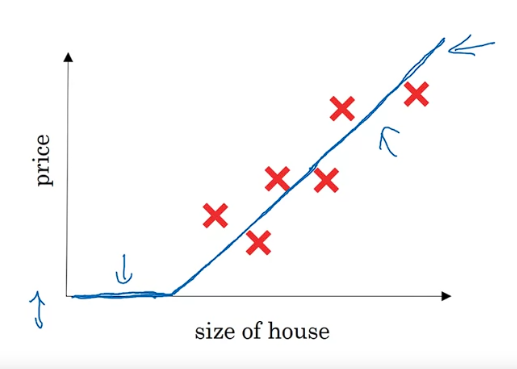
\includegraphics[width=8cm]{1.png}
        \end{figure}
        \begin{itemize}
            \item Simple neural network has a single input, neuron and output
            \item $x$: size of the house
            \item $y$: price of the house
            \item Hypothesis (blue line) is a ReLU (Rectified Linear Unit)
        \end{itemize}
        \item More complex neural networks can be formed by ``stacking'' neurons
        \begin{figure}[ht]
            \centering
            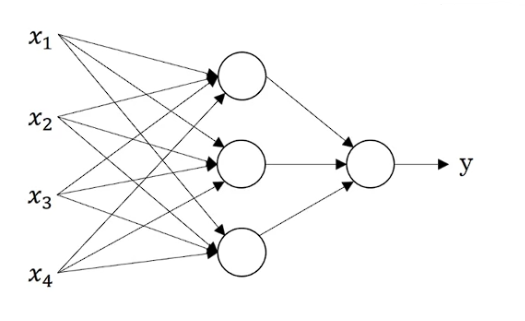
\includegraphics[width=8cm]{2.png}
        \end{figure}
        \item Every input layer feature is interconnected with every hidden layer feature
        \begin{itemize}
            \item The neural network will decide what the intermediate features will be
        \end{itemize}
        \item Most useful in supervised learning settings
    \end{itemize}
    \hspace{3mm}
    \subsubsection{Supervised Learning}
    \begin{itemize}
        \item Aims to learn a function to map an input $x$ to an output $y$
        \begin{itemize}
            \item Real estate: predicting house prices from the house features
            \item Online advertising: showing ads based on probability of user clicking on ad
            \item Photo tagging: tagging images based on objects in the image
            \item Speech recognition: generating a text transcript from audio
            \item Machine translation: translating from one language to another
            \item Autonomous driving: returning the positions of other cars from images and radar info
        \end{itemize}
        \item Different types of neural network used for different tasks
        \begin{itemize}
            \item Standard neural network: real estate and online advertising
            \item Convolutional neural network (CNN): image data
            \item Recurrent neural network (RNN): audio and language data (sequenced data)
            \item Hybrid neural network: Autonomous driving (more complex input)
        \end{itemize}
        \begin{figure}[ht]
            \centering
            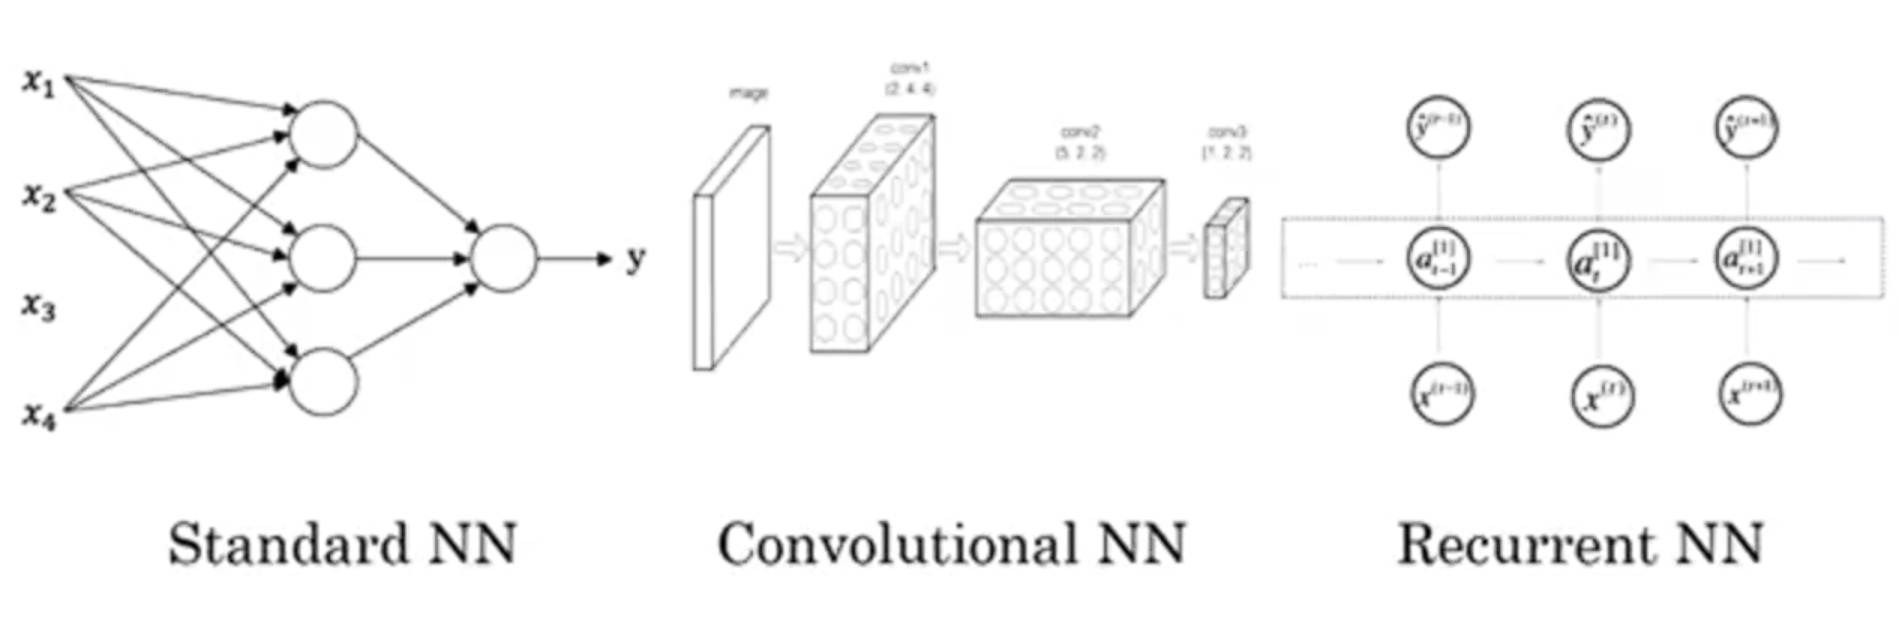
\includegraphics[width=10cm]{3.png}
        \end{figure}
        \item Supervised learning can be applied to structured and unstructured data
        \begin{itemize}
            \item Structured data has features with well defined meanings 
            \item Unstructured data has more abstract features (images, audio, text)
        \end{itemize}
    \end{itemize}

    \hspace{30mm}
    \begin{itemize}
        \item Deep learning has only recently started to become more widespread
        \begin{itemize}
            \item Given large amounts of data and a large NN, deep learning will outperform more traditional learning algorithms
            \item For small amounts of data, any performance of the algorithm depends on specific implementation
        \end{itemize}
        \begin{figure}[ht]
            \centering
            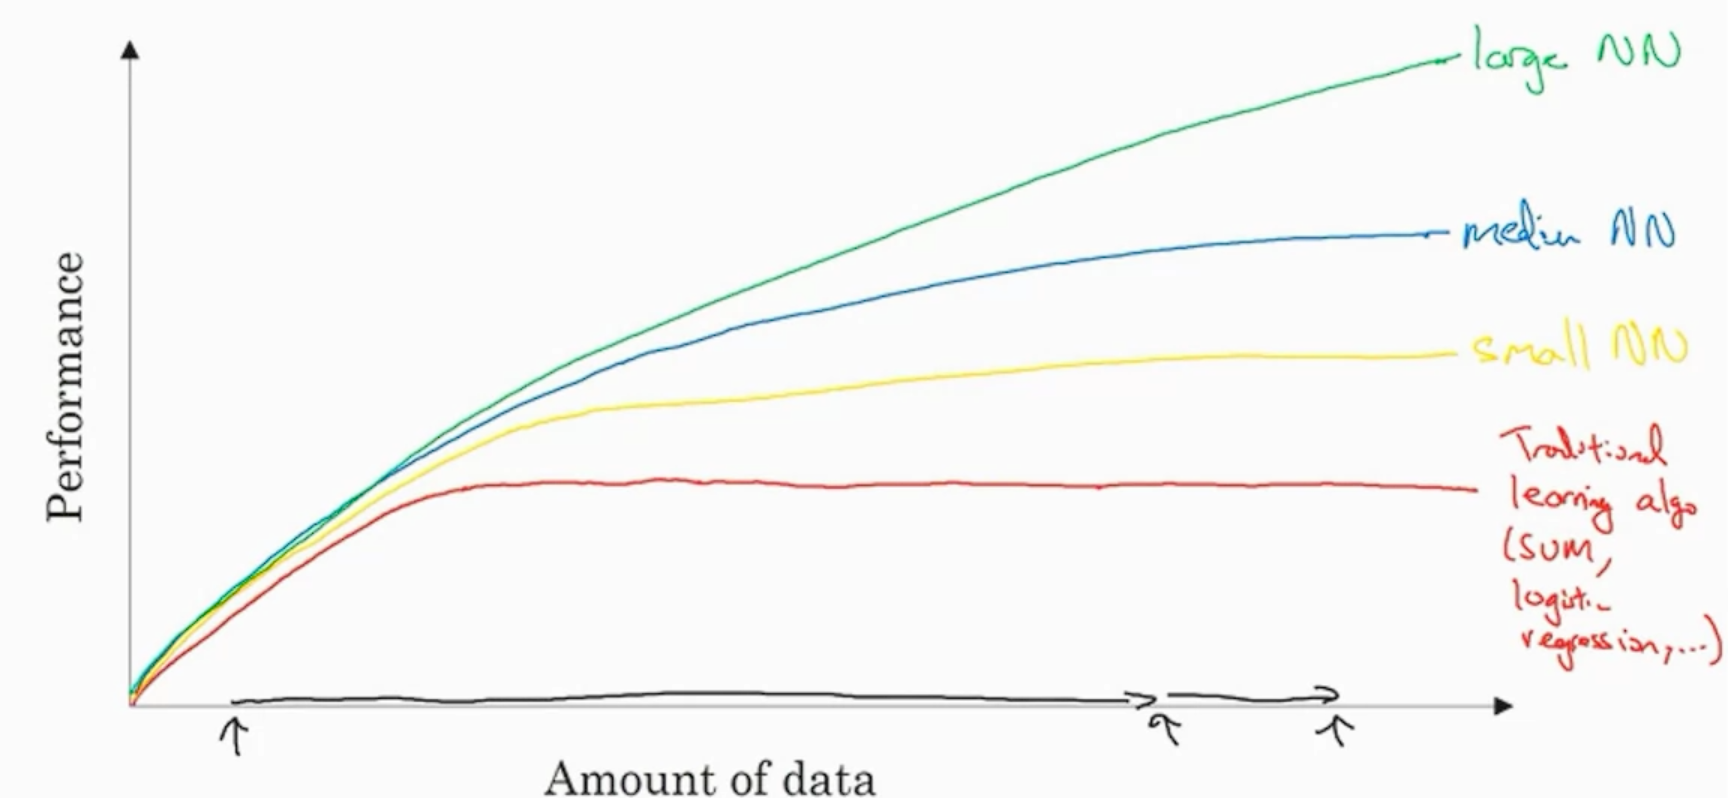
\includegraphics[width=8cm]{4.png}
        \end{figure}
        \item ``Scale drives deep learning progress''
        \begin{itemize}
            \item Both the scale of the data and the NN
        \end{itemize}
        \item Recent algorithmic innovations with increase scale of computation
        \begin{itemize}
            \item Idea to switch from sigmoid activation function to ReLu function increased NN performance
            \item Ends of sigmoid function have close to 0 gradient so and therefore result in small changes in $\theta$
            \item ReLu function has gradient of 1 for positive values
        \end{itemize}
        \item Neural network process is iterative
        \begin{itemize}
            \item Increasing speed at which a NN can be trained allows different ideas to be tried
        \end{itemize}
    \end{itemize}
    \subsection{Neural Network Basics}
    \subsubsection{Logistic Regression as a Neural Network}
    \begin{itemize}
        \item Logistic regression used for binary classification
        \item For a colour image, of 64$\times$64 pixels, will have total 12288 input features
        \begin{itemize}
            \item Image is stored as 3 separate matrices for each colour channel
            \item All pixel intensities should be unrolled into a single feature vector
            $$n=12288$$
            $$x\in\R^{12288}$$
            \item For a matrix \texttt{X} of shape $(a,b,c,d)$, want a matrix \texttt{X\_flatten} of shape $(b*c*d,1)$
        \end{itemize}
        \begin{minted}{Python}
            X_flatten = X.reshape(X.shape[0], -1).T
        \end{minted}
        
    \end{itemize}
    
    \vspace{5mm}
    \textbf{Notation} 
    $$\{(x^{(1)},y^{(1)}),(x^{(2)},y^{(2)}),...,(x^{(m)},y^{(m)})\}$$
    \begin{itemize}
        \item $(x,y)$: single training example
        \begin{itemize}
            \item $x\in\R^{n_x}$ ($n_x=$ number of features)
            \item $y\in\{0,1\}$
        \end{itemize}
        \item $(x^{(i)},y^{(i)})$: $i^{th}$ training example
        \item $m=m_{train}$
        \item $m_{test}=$ \# of test examples
        \item $X=\begin{bmatrix}
            \mid & \mid & & \mid \\
            x^{(1)} & x^{(2)} & ... & x^{(3)} \\
            \mid & \mid & & \mid \\
        \end{bmatrix}$
        \begin{itemize}
            \item $X\in\R^{n_x\times n}$
        \end{itemize}
        \item $Y=\begin{bmatrix}
            y^{(1)} & y^{(2)} & ... & y^{(m)}
        \end{bmatrix}$
        \begin{itemize}
            \item $Y\in\R^{1\times m}$
        \end{itemize}
    \end{itemize}

    \vspace{5mm}
    \textbf{Logistic Regression}
    \begin{itemize}
        \item Given $x$, want $\hat{y}=P(y=1|x)$
        \begin{itemize}
            \item Since $\hat{y}$ is a probability, want $0\leq\hat{y}\leq1$
        \end{itemize}
        \item Parameters: $w\in\R^{n_x}, b\in\R$
        \item Output: $\hat{y}=\sigma(w^Tx+b)$
        \begin{figure}[ht]
            \centering
            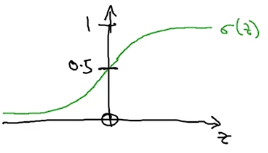
\includegraphics[width=8cm]{5.png}
        \end{figure}
        $$\sigma(z)=\frac{1}{1+e^{-z}}$$
        $$z=w^Tx+b$$
        \item Aim is to learn parameters $w$ and $b$ such that $\hat{y}$ is a good estimate of the probability
        \item Previous convention had $\theta$ vector with an additional $\theta_0$ parameter
        \begin{itemize}
            \item Keeping $\theta_0$ ($b$) separate from the rest of the parameters is easier to implement
        \end{itemize}
    \end{itemize}

    \vspace{3mm}
    \textbf{\textit{Cost Function}}
    \begin{itemize}
        \item Given $\{(x^{(1)}, y^{(1)}),(x^{(2)}, y^{(2)}), ..., (x^{(m)}, y^{(m)})\}$, want $\hat{y}^{(i)} \approx y^{(i)}$
        \item Squared error function not used for logistic regression loss function 
        \begin{itemize}
            \item Optimization problem becomes non convex and will have local optima
        \end{itemize}

        \vspace{10mm}
        $$\mathcal{L}(\hat{y},y)=-(y\log(\hat{y})+(1-y)\log(1-\hat{y}))$$
        \item If $y=1$:
        \begin{itemize}
            \item $\mathcal{L}(\hat{y},y)=-\log(\hat{y})$
            \item Want large $\log(\hat{y})$ $\therefore$ want large $\hat{y}$
            \item $\hat{y}$ has a max of 1 $\therefore$ want $\hat{y}=1$
        \end{itemize}
        \item If $y=0$:
        \begin{itemize}
            \item $\mathcal{L}(\hat{y}, y)=-log(1-\hat{y})$
            \item Want large $\log(1-\hat{y})$ $\therefore$ want small $\hat{y}$
            \item $\hat{y}$ has a min of 0 $\therefore$ want $\hat{y}=0$
        \end{itemize}
        \item Cost function:
        \begin{align*}
            J(w,b)&=\frac{1}{m}\sum_{i=1}^{m}\mathcal{L}(\hat{y}^{(i)},y^{(i)}) \\
            &= -\frac{1}{m}\sum_{i=1}^{m}[y^{(i)}\log(\hat{y}^{(i)})+(1-y^{(i)})\log(1-\hat{y}^{(i)})]
        \end{align*}
        \begin{itemize}
            \item Average loss function over all training examples
        \end{itemize}
    \end{itemize}

    \vspace{3mm}
    \textbf{\textit{Gradient Descent}}
    \begin{itemize}
        \item Want to find values of $w$ and $b$ that minimize the cost function $J(w,b)$
        \begin{itemize}
            \item For logistic regression, $w$ and $b$ usually initialized to 0
        \end{itemize} 
        \item One iteration of gradient descent will take a step in the direction of steepest descent
    \end{itemize}

    \vspace{3mm}
    \begin{lstlisting}
    Repeat {
        w := w - $\alpha \frac{\partial J(w,b)}{\partial w}$
        b := b - $\alpha \frac{\partial J(w,b)}{\partial b}$
    }  
    \end{lstlisting}
    \begin{itemize}
        \item Using the computation graph:
        \begin{figure}[ht]
            \centering
            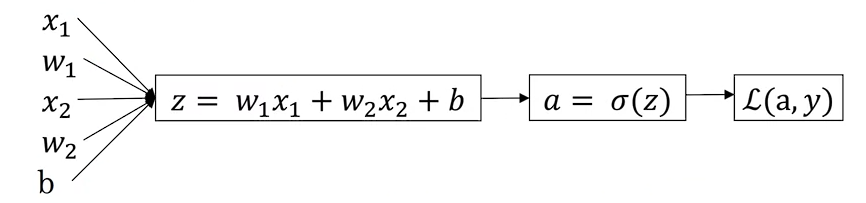
\includegraphics[width=12cm]{6.png}
        \end{figure}
        \begin{center}
            $$\frac{\partial \mathcal{L}(a,y)}{\partial a}=-\frac{y}{a}+\frac{1-y}{1-a}$$
            \begin{align*}
                \frac{\partial\mathcal{L}(a,y)}{\partial z} &=\frac{\partial\mathcal{L}}{\partial a} \times \frac{\partial a}{\partial z} \\
                &= (-\frac{y}{a}+\frac{1-y}{1-a}) \times a(1-a) \\
                &= a-y
            \end{align*}
            $$\frac{\partial\mathcal{L}}{\partial w_1}=x_1 \times \frac{\partial\mathcal{L}}{\partial z}$$
            $$\frac{\partial\mathcal{L}}{\partial w_2}=x_2 \times \frac{\partial\mathcal{L}}{\partial z}$$
            $$\frac{\partial\mathcal{L}}{\partial b}=\frac{\partial\mathcal{L}}{\partial z}$$
        \end{center}
        \item Partial derivative over all training examples calculated by taking the average \texttt{dw1}
        $$\frac{\partial}{\partial w_1}J(w,b)=\frac{1}{m}\sum^m_{i=1}\frac{\partial}{\partial w_1} \mathcal{L}(a^{(i)},y^{(i)})$$

        Initialize \texttt{J = 0, dw1 = 0, dw2 = 0, db = 0}
        \begin{lstlisting}
        For i = 1 to m:
            z$^{(i)}$ = w$^T$x$^{(i)}$ + b
            a$^{(i)}$ = $\sigma$(z$^{(i)}$)

            J += -[y$^{(i)}$ $\log$(a$^{(i)}$) + (1-y$^{(i)}$)$\log$(1-a$^{(i)}$)]
            dz$^{(i)}$ = a$^{(i)}$ - y$^{(i)}$
            dw1 += x$_1^{(i)}$ dz$^{(i)}$
            dw2 += x$_2^{(i)}$ dz$^{(i)}$
            db += dz$^{(i)}$

        J /= m
        dw1 /= m
        dw2 /= m
        db /= m

        w1 := w1 - $\alpha$ dw1
        w2 := w2 - $\alpha$ dw2 
        b := b - $\alpha$ db
        \end{lstlisting}
        \item Above implementation requires \texttt{for} loop over all features for all training examples
        \begin{itemize}
            \item Vectorization can be used to remove explicit \texttt{for} loops
            \item Vectorization required for deep learning to be efficient
        \end{itemize}
    \end{itemize}

    \subsubsection{Vectorisation in Python}
    \begin{itemize}
        \item Deep learning performs best on large data sets
        \begin{itemize}
            \item Code must be able to run quickly to be effective on large data sets
        \end{itemize}
        $$z=w^Tx + b$$
        $$w\in \R^{n_x} ~~ x\in \R^{n_x}$$
        \item Non vectorized implementation:
        \begin{minted}{Python}
            z = 0
            for i in range(n_x):
                z += w[i] * x[i]
            z += b
        \end{minted}
        \item GPUs and CPUs both have parallelization instructions (SIMD: Single Instruction Multiple Data)
        \begin{itemize}
            \item If built in functions are used, \texttt{numpy} will use parallelism to perform computations faster 
        \end{itemize}
        \item For logistic regression, need to calculate $z$ and $a$ values for each training example
        $$z^{(i)}=w^Tx^{(i)}+b$$
        $$a^{(i)}=\sigma(z^{(i)})$$
        $$X = \begin{bmatrix}
            \mid & \mid & & \mid \\
            x^{(1)} & x^{(2)} & ... & x^{(m)} \\
            \mid & \mid & & \mid 
        \end{bmatrix} $$
        $$w\in\R^{n_x} ~~ X\in\R^{n_x\times m}$$ 
        \begin{align*}
            \begin{bmatrix}
                z^{(1)} & z^{(2)} & ... & z^{(m)}
            \end{bmatrix}
            &= w^TX + \begin{bmatrix}
                b & b & ... & b
            \end{bmatrix} \\
            &= \begin{bmatrix}
                w^Tx^{(1)}+b & w^Tx^{(2)}+b & ... & w^Tx^{(m)}+b 
            \end{bmatrix}
        \end{align*}
        \item In Python:
        \begin{minted}{Python}
            Z = np.dot(w.T, X) + b
        \end{minted}
        \begin{itemize}
            \item Python will broadcast the value \texttt{b} so it can be added to the matrix
        \end{itemize}
        \item Vectorized implementation of sigmoid function can be used on \texttt{Z} to calculate \texttt{A}
        $$A= \begin{bmatrix}
            a^{(1)} & a^{(2)} & ... & a^{(m)}
        \end{bmatrix} $$
        
        $$dz^{(i)}=a^{(i)}-y^{(i)}$$
        $$dz=A-Y$$
        $$db=\frac{1}{m}\sum^m_{i=1}dz^{(i)}$$
        $$dw=\frac{1}{m}X(dz)^T$$
        \begin{minted}{Python}
            Z = np.dot(w.T,X) + b
            A = sigmoid(Z)
            dz = A - Y
            dw = 1/m * np.dot(X, dz.T)
            db = 1/m * np.sum(dz)

            # Gradient descent update
            w = w - alpha * dw
            b = b - alpha * db
        \end{minted}
        \item \texttt{for} loop is required to run multiple iterations of gradient descent
    \end{itemize}
    \subsection{Shallow Neural Networks}
    \begin{itemize}
        \item A neural network will have stacked logistic regression units in each layer
        \begin{itemize}
            \item Logistic regression output from one layer will be fed to another layer
        \end{itemize}
    \end{itemize}

    \vspace{25mm}
    \begin{itemize}
        \begin{figure}[ht]
            \centering
            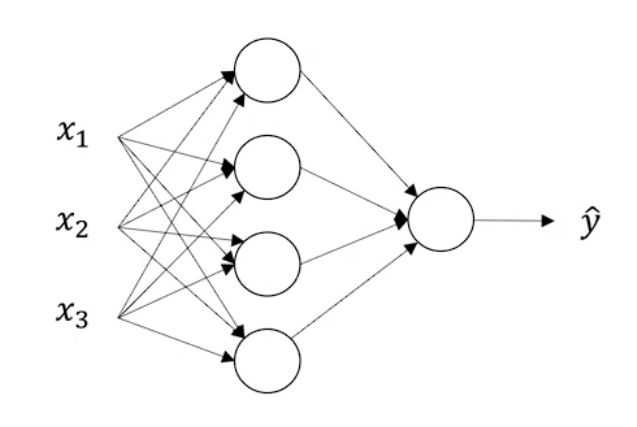
\includegraphics[width=8cm]{7.png}
        \end{figure}
        \item Input layer of the neural network contains the feature $x_1, x_2, x_3$
        \begin{itemize}
            \item $a^{[0]}=X$    
        \end{itemize}
        \item Intermediate layers in the network are hidden layers
        \begin{itemize}
            \item Hidden layers do not have ``true'' values in the training set
        \end{itemize}
        \item Final layer in the network is the output layer
        \begin{itemize}
            \item Generates the predicted value $\hat{y}$
        \end{itemize}
        \item Above diagram is a 2 layer NN
        \begin{itemize}
            \item Input layer is layer 0
        \end{itemize}
        \item Each layer will have parameters $w$ and $b$ associated with them 
        \item Each node in the NN will perform logistic regression with its inputs
        $$z_i^{[l]}=w_i^{[l]T}x+b_i^{[l]} ~~\rightarrow~~ a_i^{[l]}=\sigma(z_i^{[l]})$$
      

        $$W^{[1]} = \begin{bmatrix}
            - & w_1^{[1]T} & - \\
            - & w_2^{[1]T} & - \\
            - & w_3^{[1]T} & - \\
            - & w_4^{[1]T} & - 
        \end{bmatrix} $$
        $$a^{[0]}=\begin{bmatrix}
            x_1 \\
            x_2 \\
            x_3
        \end{bmatrix} $$
        $$b^{[1]}=\begin{bmatrix}
            b_1^{[1]} \\
            b_2^{[1]} \\
            b_3^{[1]} \\
            b_4^{[1]} 
        \end{bmatrix}$$

        \begin{align*}
            z^{[1]}&=\begin{bmatrix}
                z_1^{[1]} \\
                z_2^{[1]} \\
                z_3^{[1]} \\
                z_4^{[1]} \\
            \end{bmatrix} \\
            &= \begin{bmatrix}
                w_1^{[1]T}a^{[0]}+b_1^{[1]} \\
                w_2^{[1]T}a^{[0]}+b_1^{[1]} \\
                w_3^{[1]T}a^{[0]}+b_1^{[1]} \\
                w_4^{[1]T}a^{[0]}+b_1^{[1]} \\
            \end{bmatrix} \\
            &= w^{[1]} a^{[0]} + b^{[1]}
        \end{align*}

        \begin{align*}
            a^{[1]}&=\begin{bmatrix}
                a_1^{[1]} \\
                a_2^{[1]} \\
                a_3^{[1]} \\
                a_4^{[1]} \\
            \end{bmatrix} \\
            &= \sigma(z^{[1]})
        \end{align*}
        $$z^{[2]}=W^{[2]}a^{[1]}+b^{[2]} ~~\rightarrow~~ a^{[2]}=\sigma(z^{[2]})$$
    \end{itemize}

    \begin{itemize}
        \item Vectorized method should be able to work on all training examples at one time
        \begin{itemize}
            \item Vector for each training example can be stacked horizontally in a matrix
            \item Vertical dimension will be the number of units in a layer ($n_x$ for the input layer)
        \end{itemize}
    \end{itemize}

    $$X=\begin{bmatrix}
        \mid & \mid & & \mid \\
        x^{(1)} & x^{(2)} & & x^{(m)} \\
        \mid & \mid & & \mid
    \end{bmatrix}$$

    $$Z^{[1]}=\begin{bmatrix}
        \mid & \mid & & \mid \\
        z^{[1](1)} & z^{[1](2)} & ... & z^{[1](m)} \\
        \mid & \mid & & \mid
    \end{bmatrix}$$

    $$A^{[1]}=\begin{bmatrix}
        \mid & \mid & & \mid \\
        a^{[1](1)} & a^{[1](2)} & ... & a^{[1](m)} \\
        \mid & \mid & & \mid
    \end{bmatrix}$$
    
    \begin{align*}
        Z^{[1]}&=W^{[1]}X+b^{[1]} \\
        A^{[1]}&=\sigma(Z^{[1]}) \\
        Z^{[2]}&=W^{[2]}A^{[1]}+b^{[2]} \\
        A^{[2]}&=\sigma(Z^{[2]})
    \end{align*}

    \subsubsection{Activation Functions}
    \begin{itemize}
        \item After $z$ values are calculated, activation function must be run to get the activation value $a$
        $$a_{sigmoid}=\frac{1}{1+e^{-z}}$$
        \item Alternatively $a^{[1]}=g(z^{[1]})$ where $g$ is a non linear function
        \item $\tanh$ function almost always performs better than the sigmoid function
        \begin{itemize}
            \item Equivalent to a transformed version of the sigmoid function  
            \item $\tanh$ function is odd and is ``centered'' around the origin
            \item The mean of the data will be closer to 0 and will help with learning in the next layer
        \end{itemize}
        $$a_{\tanh}=\frac{e^z-e^{-z}}{e^z+e^{-z}}$$
        \begin{figure}[ht]
            \centering
            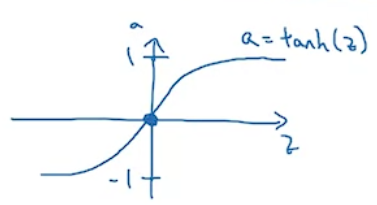
\includegraphics[width=8cm]{8.png}
        \end{figure}
        \item For binary classification, the final output layer can use the sigmoid function
        \begin{itemize}
            \item Want the value of $\hat{y}$ to be between 0 and 1
        \end{itemize}
        \item For both the sigmoid and $\tanh$ functions, when $z$ is large, the gradient is very small
        \begin{itemize}
            \item Results in a slower gradient descent
        \end{itemize}
        \item ReLU function has a gradient of 1 when $z$ is positive
        \begin{figure}[ht]
            \centering
            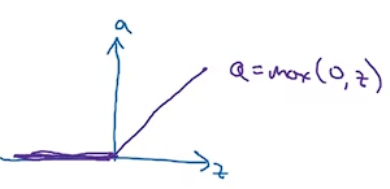
\includegraphics[width=8cm]{9.png}
        \end{figure}
        \begin{itemize}
            \item Gradient is 0 when $z$ is negative
        \end{itemize}
        \item For majority of the ReLU function, gradient is very different from 0
        \begin{itemize}
            \item Will typically allow NN to learn much faster than sigmoid or $\tanh$ function
        \end{itemize}
        \item ReLU function should be used as the default activation function
        \item The leaky ReLu function has a slight positive gradient when $z$ is negative
        $$a_{leaky ReLU}=\max(0.01z, z)$$
        \begin{figure}[ht]
            \centering
            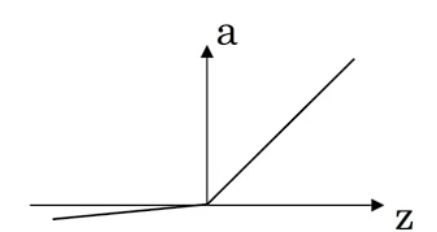
\includegraphics[width=8cm]{10.png}
        \end{figure}
        \item For a NN to compute more complex functions, activation function must be non linear
        \begin{itemize}
            \item If a linear activation function is used, final output of the NN can only be a linear function 
            \item Multiple linear activation neurons with a sigmoid as the output neuron is equivalent to standard logistic regression
        \end{itemize}
        \item Linear activation function can be used in the output layer if output is a real number
        \item Derivative of the activation function must be calculated for backpropagation
        \begin{itemize}
            \item Sigmoid function
            $$g(z)=\frac{1}{1+e^{-z}}$$
            \begin{align*}
                \frac{d}{dz}g(z)&=\frac{1}{1+e^{-z}}\left(1-\frac{1}{1+e^{-z}}\right) \\
                &=g(z)(1-g(z))
            \end{align*}
            \item $\tanh$ function
            \begin{align*}
            g(z)&=\tanh(z) \\
            &=\frac{e^z-e^{-z}}{e^z+e^{-z}}
            \end{align*}
            \begin{align*}
                \frac{d}{dz}g(z)&=1-\left(\frac{e^z-e^{-z}}{e^z+e^{-z}}\right)^2 \\
                &=1-g(z)^2
            \end{align*}
            \item ReLU function
            $$g(z)=\max(0,z)$$
            $$\frac{d}{dz}g(z)=\begin{cases}
                0 & \text{if } z < 0 \\
                1 & \text{if } z \geq 0
            \end{cases}$$
            \item Leaky ReLU function
            $$g(z)=\max(0.01z,z)$$
            $$\frac{d}{dz}g(z)=\begin{cases}
                0.01 & \text{if } z < 0 \\
                1 & \text{if } z \geq 0
            \end{cases}$$
        \end{itemize}

    \end{itemize}
    \subsubsection{Gradient Descent for Neural Networks}
    \begin{itemize}
        \item For a single hidden layer NN, parameters are: $w^{[1]}, b^{[1]}, w^{[2]}, b^{[2]}$
        \begin{itemize}
            \item $w^{[1]}\in\R^{n_1\times n_0}$
            \item $b^{[1]}\in\R^{n_1\times 1}$
            \item $w^{[2]}\in\R^{n_2\times n_1}$
            \item $b^{[2]}\in\R^{n_2\times 1}$
        \end{itemize}
        \item Cost function: $J(w^{[1]}, b^{[1]}, w^{[2]}, b^{[2]})=\frac{1}{m}\sum_{i=1}^n\mathcal{L}(\hat{y},y)$
        \item For one iteration of gradient descent:
        $$w^{[1]}:=w^{[1]}-\alpha dw^{[1]},~b^{[1]}:=b^{[1]}-\alpha db^{[1]}$$
        $$w^{[2]}:=w^{[2]}-\alpha dw^{[2]},~b^{[2]}:=b^{[2]}-\alpha db^{[2]}$$
        \begin{itemize}
            \item Gradient descent step will take place after backpropagation calculates the derivatives
        \end{itemize}
        \item Forward propagation:
        \begin{align*}
            Z^{[1]}&=W^{[1]}X+b^{[1]} \\
            A^{[1]}&=g^{[1]}(Z^{[1]}) \\
            Z^{[2]}&=W^{[2]}A^{[1]}+b^{[2]} \\
            A^{[2]}&=g^{[2]}(Z^{[2]})
        \end{align*}
        \item Backpropagation:
        \begin{align*}
            dz^{[2]}&=A^{[2]}-Y \\
            dw^{[2]}&=\frac{1}{m}dz^{[2]}A^{[1]T} \\
            db^{[2]}&=\frac{1}{m}\texttt{np.sum}(dz^{[2]}, \texttt{axis = 1, keepdims = True}) \\
            dz^{[1]}&=w^{[2]T}dz^{[2]}\times g^{[1]'}(z^{[1]}) \\
            dw^{[1]}&=\frac{1}{m}dz^{[1]}X^T \\
            db^{[1]}&=\frac{1}{m}\texttt{np.sum}(dz^{[1]}, \texttt{axis = 1, keepdims = True})
        \end{align*}
    \end{itemize} 

    \subsubsection{Random Initialization}
    \begin{itemize}
        \item Weights must be initialized randomly for a NN
        \begin{itemize}
            \item Weights can be initialized to 0 for logistic regression
            \item The bias terms $b$ can be initialized
        \end{itemize}
        \item If weights are initialized to 0, all neurons in a layer will compute the same hypothesis
        \begin{minted}{Python}
            W1 = np.random.randn((2,2)) * 0.01
            b1 = np.zero((2,1))  
        \end{minted}
        \item Weights should be initialized to small random values
        \begin{itemize}
            \item If weight is too large, activation value $z^{[1]}$ will be large
            \item If sigmoid or $\tanh$ function is used, derivative will be very small and learning will be very slow
        \end{itemize}
        \item Different constant for \texttt{np.random.randn} should be used for deeper neural networks
    \end{itemize}
    \subsection{Deep Neural Networks}
    \begin{itemize}
        \item Logistic regression is equivalent to a 1-layer NN
        \item Deep NN have more hidden layers
        \begin{itemize}
            \item Number of hidden layers in the network can be a parameter for the ML problem
        \end{itemize}
        
        \vspace{25mm}
        \begin{figure}[ht]
            \centering
            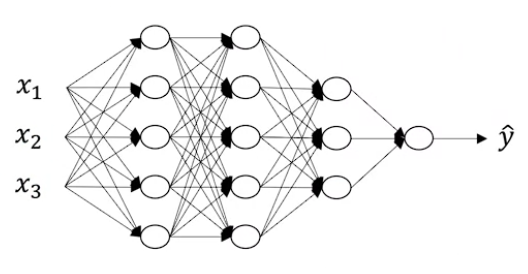
\includegraphics[width=8cm]{11.png}
        \end{figure}
        \begin{itemize}
            \item Above network has 4 layers, $L=4$
            \item $n^{[l]}=$ number of units in layer $l$
            \item $a^{[l]}=$ activations in layer $l$
        \end{itemize}
        \item The inputs $x$ are the activations of the first layer, $x=a^{[0]}$
        \begin{itemize}
            \item Prediction $\hat{y}$ will be the activations of the last layer, $\hat{y}=a^{[L]}$
        \end{itemize}
        \item Forward propagation for a deep NN will follow the same pattern for all layers
        $$z^{[l]}=w^{[l]}a^{[l-1]}+b^{[l]}$$
        $$a^{[l]}=g^{[l]}(z^{[l]})$$
        \item For a vectorized implementation
        $$Z^{[l]}=W^{[l]}A^{[l-1]}+b^{[l]}$$
        $$A^{[l]}=g^{[l]}(z^{[l]})$$
        \begin{itemize}
            \item Explicit for loop will be used to loop over the layers in the network
            \item $b$ will still be a column vector but will apply correctly due to broadcasting
            \item When working with $W$ and $A$ matrices, $A$ will be for the previous layer so the dimensions will fit
        \end{itemize}
        \item When debugging NN, can look at dimensions of all the matrices
        \item For a non vectorized implementation:
        \begin{itemize}
            \item $W^{[l]}:(n^{[l]},n^{[l-1]})$
            \item $b^{[l]}:(n^{[l]},1)$
            \item Dimensions of $dw$ and $db$ should be the same as the dimensions of $W$ and $b$
            \item $a^{[l]}, z^{[l]}:(n^{[l]},1)$ 
        \end{itemize}
        \item For a vectorized implementation, $z$ vectors and $a$ vectors will be stacked horizontally for all training examples
        \begin{itemize}
            \item $Z^{[l]},A^{[l]}:(n^{[l]},m)$
        \end{itemize}
        \item Deep NN tend to work better as each layer can compute increasingly complex functions
        \begin{itemize}
            \item Face recognition: edge detection $\rightarrow$ individual features $\rightarrow$ large parts of the face
            \item Audio: low level waveforms $\rightarrow$ phonemes $\rightarrow$ words $\rightarrow$ sentences
        \end{itemize}
        \item Functions that can be computed with a ``small'' deep neural network require exponentially more hidden units in a shallower network
        \item For each forward propagation step, the value of $z^{[l]}$ should be cached for backpropagation
        \begin{itemize}
            \item Values of $w^{[l]}$ and $b^{[l]}$ can also be stored in the cache so they can be accessed for backpropagation
        \end{itemize}
        \begin{figure}[ht]
            \centering
            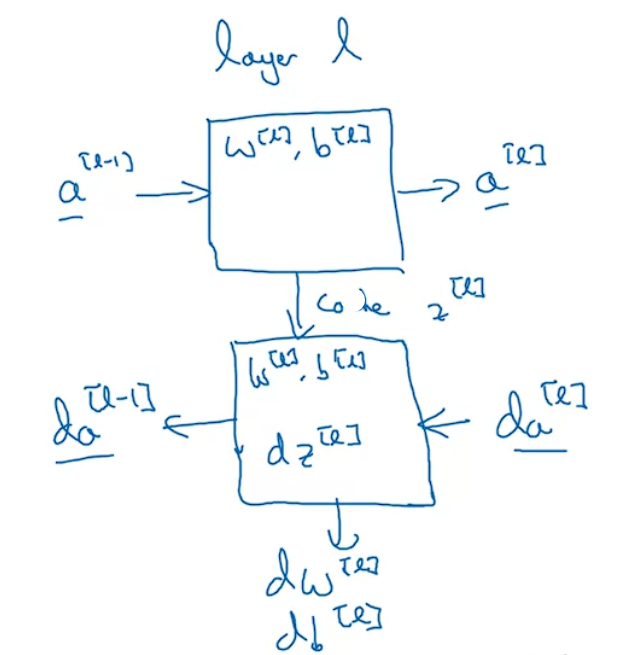
\includegraphics[width=8cm]{12.png}
        \end{figure}
        \item All forward propagation steps will carried out until the hypothesis, $\hat{y}$ is found
        \begin{itemize}
            \item Using cached values, all backpropagation steps will be carried out until $dz^{[1]}$
            \item Parameters $W^{[l]}$ and $b^{[l]}$ can be updated accordingly
            $$W^{[l]}:=W^{[l]}-\alpha dw^{[l]}$$
            $$b^{[l]}:=b^{[l]}-\alpha db^{[l]}$$
        \end{itemize}
        \item Backpropagation will also follow a pattern for all layers in the NN
        \begin{itemize}
            \item $dz^{[l]}=da^{[l]}*g^{[l]'}(z^{[l]})$
            \item $dW^{[l]}=dz^{[l]}a^{[l-1]T}$
            \item $db^{[l]}=dz^{[l]}$
            \item $da^{[l-1]}=W^{[l]T}dz^{[l]}$
        \end{itemize}
        \item For a vectorized implementation:
        \begin{itemize}
            \item $dZ^{[l]}=dA^{[l]}*g^{[l]'}(Z^{[l]})$
            \item $dW^{[l]}=\frac{1}{m}dZ^{[l]}A^{[l-1]T}$
            \item $db^{[l]}=\frac{1}{m}\texttt{np.sum}(dZ^{[l]}\texttt{, axis=1, keepdims=True})$
            \item $dA^{[l-1]}=W^{[l]T}dZ^{[l]}$
        \end{itemize}
    \end{itemize}
    \subsubsection{Parameters vs Hyperparameters}
    \begin{itemize}
        \item Parameters of the NN are the $W$ and $b$ matrices
        \item NN also has a number of associated hyperparameters:
        \begin{itemize}
            \item Learning rate $\alpha$
            \item Number of iterations z`'
            \item Number of layers in the network
            \item Number of hidden units
            \item Choice of activation function
        \end{itemize}
        \item Hyperparameters will control the values of $W$ and $b$
        \item Deep learning has many more hyperparameters than earlier eras of machine learning
        \begin{itemize}
            \item Applying deep learning becomes an empirical process
        \end{itemize}
        \item Intuitions about hyperparameters may be different across different applications
    \end{itemize}
    \pagebreak

    \section{Improving Deep Neural Networks: Hyperparameter Tuning, Regularization and Optimization}
    \subsection{Practical Aspects of Deep Learning}
    \begin{itemize}
        \item Applying ML is a highly iterative process
        \begin{itemize}
            \item Very hard to choose ``correct'' values for hyperparameters
        \end{itemize}
        \begin{figure}[ht]
            \centering
            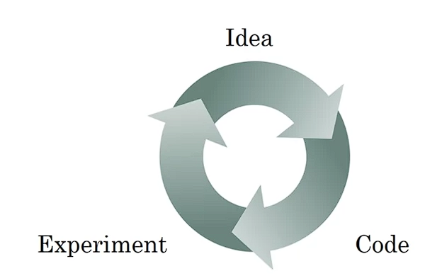
\includegraphics[width=8cm]{13.png}
        \end{figure}
        \item Deep learning used in many different areas
        \begin{itemize}
            \item NLP
            \item Computer vision 
            \item Speech analysis
            \item Structured data
            \begin{itemize}
                \item Advertisement
                \item Search engines
                \item Computer security
                \item Logistics 
            \end{itemize}
        \end{itemize}
        \item Intuitions from one subject area often don't transfer to another application
        \item Success of deep learning can depend on speed of iteration
        \begin{itemize}
            \item Choice of split of the data can influence speed of iteration
        \end{itemize}
        \item Whole dataset should be split into training, development and test set
        \begin{itemize}
            \item Dev set should be used rate performance of different models
            \item Final model should be evaluated on the test set
            \item Split will allow better evaluation of bias and variance of the model
        \end{itemize}
        \item Previous eras of ML had a 60/20/20 split between dataset
        \item For the big data era, a smaller percentage of data is given to the dev and test sets
        \begin{itemize}
            \item For 1,000,000 examples, can allocate just 10,000 examples each to dev and test set
            \item 10,000 examples is enough to run the algorithm and get a good idea about the algorithm performance
        \end{itemize}
        \item Recent trends also show mismatched training and test set distributions
        \begin{itemize}
            \item For images, training set may have very high quality images while test set may have lower quality
            \item Dev and test set should come from the same distribution
        \end{itemize}
        \item Dataset might be split to not include a test set
        \begin{itemize}
            \item Dev set can be used to get to a ``good'' model
            \item Since data is fit to the dev set, there is no unbiased estimate of performance
            \item When data doesn't include a test set, dev set is usually referred to as ``test'' set 
        \end{itemize}
    \end{itemize}
    \subsubsection{Bias and Variance}
    \begin{itemize}
        \item In the deep learning era, there tends to be less of a discussion about the bias/variance trade off
        \item In 2 dimensions, data can be plotted to look for high bias or variance
        \begin{itemize}
            \item High bias classifiers underfit the data
            \item High variance classifiers overfit the data
        \end{itemize}
        \item For higher dimensions, training set error and dev set error can be used
        \begin{itemize}
            \item High variance classifier has low training error and high dev set error
            \item High bias classifier has high training error and high dev set error
            \item Classifier with high bias and high variance will have high training error and even higher dev set error
        \end{itemize}
        \item Above ideas only work with the assumption that the optimal error is 0\%
        \begin{itemize}
            \item Training and dev set must also come from the same distribution
        \end{itemize}
    \end{itemize}
    \subsubsection{Basic Recipe for Machine Learning}
    \begin{itemize}
        \item Train initial algorithm and reduce bias of algorithm to an ``acceptable value''
        \begin{itemize}
            \item Use a larger network 
            \item Train algorithm for longer
        \end{itemize}
        \item Reduce variance of the algorithm by getting more data
        \begin{itemize}
            \item Add regularization terms to the cost function
        \end{itemize}
        \item Bias and variance can also be reduced by using a more appropriate NN architecture
        \item In the big data era, bias and variance can be reduced without affecting each other
        \begin{itemize}
            \item Training a bigger network typically reduce the bias 
            \item Getting more training data will typically reduce the variance
        \end{itemize}
        \item Using regularization will have a bias variance trade off
    \end{itemize}
    \subsubsection{Regularization}
    \begin{itemize}
        \item Adding regularization will usually help in reducing variance and prevent overfitting
        \item For logistic regression:
        $$J(w,b)=\frac{1}{m}\sum_{i=1}^m\mathcal{L}(\hat{y}^{(i)}, y^{(i)})+\frac{\lambda}{2m}||w||_2^2$$
        \begin{align*}
            ||w||_2^2&=\sum_{j=1}^{n_x}w_j^2 \\
            &=w^Tw
        \end{align*}
        \begin{itemize}
            \item Above method is $L_2$ regularization after the $L_2$ norm (Euclidean norm) of $w$
            \item $b$ values can also be regularized but will have a much smaller effect than $w$ 
        \end{itemize}
        \item $L_1$ regularization adds the term:
        $$\frac{\lambda}{m}\sum_{i=1}^{n_x}|w|=\frac{\lambda}{m}||w||_1$$
        \begin{itemize}
            \item Using $L_1$ regularization will result in $w$ being sparse
            \item Can be seen to compressing the model
        \end{itemize}
        \item $L_2$ regularization is more common for deep learning 
        \item Regularization parameter $\lambda$ will be set using the cross validation set
        \begin{itemize}
            \item \texttt{lambda} is a reserved keyword in Python 
        \end{itemize}
        \item For a neural network:
        $$J(w^{[1]},b^{[1]},...,w^{[l]}, b^{[l]})=\frac{1}{m}\sum_{i=1}^m\mathcal{L}(\hat{y}^{(i)}, y^{(i)})+\frac{\lambda}{2m}\sum_{l=1}^L||w^{[l]}||^2$$
        $$||w^{[L]}||^2=\sum^{n^{[l]}}_{i=1}\sum_{j=1}^{n^{[l-1]}} (w^{[l]}_{i,j})^2$$
        \begin{itemize}
            \item $||W^{[l]}||^2_F$ known as the Frobenius norm of the matrix
        \end{itemize}
        \item Since new term added to cost function, $\frac{\partial J}{\partial W^{[l]}}$ will be different
        $$dW^{[l]}=...+\frac{\lambda}{m}W^{[l]}$$
        $$W^{[l]}=W^{[l]}-\frac{\alpha\lambda}{m}W^{[l]}-\alpha(...)$$ 
        \begin{itemize}
            \item Also known as weight decay as value of $W$ will decrease on every iteration
            $$W^{[l]}-\frac{\alpha\lambda}{m}W^{[l]}=\left(1-\frac{\alpha\lambda}{m}\right)W^{[l]}$$
            \item Value of $\left(1-\frac{\alpha\lambda}{m}\right)$ will be slightly less than 1
        \end{itemize}
        \item Adding regularization term will penalize the weight matrix from being too large
        \begin{itemize}
            \item As the value of $\lambda$ is increased, the weights in $w$ will get closer to 0 
            \item Each hidden unit will have a smaller effect and the resulting NN will be simpler
        \end{itemize}
        \item When using the tanh function, penalizing $w$ will make $z^{[l]}$ smaller
        \begin{itemize}
            \item For a small $z^{[l]}$, tanh function is roughly linear
            \item If all hidden units in the network are roughly linear, the result of the NN will also be roughly linear
        \end{itemize}
    \end{itemize}

    \vspace{5mm}
    \textbf{Dropout Regularization}
    \begin{itemize}
        \item Each layer in the NN has a probability of eliminating a node
        \begin{itemize}
            \item When a node is eliminated, all outgoing links from the node are also deleted
            \item Each example will be trained on a smaller network so will have less chance of overfitting 
        \end{itemize}
        \item For each different training example, the NN is reset and randomly eliminates nodes again
        \item Inverted dropout:
        \begin{minted}{Python}
    d3 = np.random.rand(a3.shape[0], a3.shape[1]) < keep_prob
    a3 = np.multiply(a3, d3)
    a3 /= keep_prob
        \end{minted}
        \begin{itemize}
            \item For \texttt{keep\_prob} = 0.8  each node has a 0.2 chance of being removed
            \item Activation values should be scaled by \texttt{keep\_prob} so the expected value of $z$ can stay constant
            \item On each pass through the training set, a different set of units should be zeroed out   
        \end{itemize}
        \item At test time, dropout should not be used as it will create noise in the predictions
        \item A single hidden unit cannot rely on a specific feature as it may not be used on each iteration
        \begin{itemize}
            \item Weights for the unit will be spread out between the units
            \item Has the same effect as shrinking the weights like L2 regularization
            \item The equivalent L2 penalty on different weights depends on the size of the activations being used for the weight
        \end{itemize}
        \item \texttt{keep\_prob} can be varied between the layers
        \begin{itemize}
            \item Larger layers may be more prone to overfitting and can have a larger \texttt{keep\_prob}
            \item For small layers with a very small chance of overfitting, \texttt{keep\_prob} can be set to 1
        \end{itemize}
        \item Many dropout implementations started with computer vision
        \begin{itemize}
            \item Input size for computer vision is extremely large
        \end{itemize}
        \item Cost function is not well defined when dropout is used
        \begin{itemize}
            \item Can set \texttt{keep\_prob} to 1 and check for monotonically decreasing $J$
            \item When $J$ is decreasing, then can reduce the value of \texttt{keep\_prob} to use dropout
        \end{itemize}
    \end{itemize}
    
    \vspace{5mm}
    \textbf{Other Regularization Methods}
    \begin{itemize}
        \item Getting more training data will almost always help overfitting
        \begin{itemize}
            \item May not be possible to get more training data or very expensive
        \end{itemize}
        \item Data augmentation will create new examples and can help reduce overfitting
        \item For an image dataset:
        \begin{itemize}
            \item Flipping the image horizontally
            \item Randomly cropping and distorting the image
        \end{itemize}
        \item Magnitude of image transformation depends on classifier
        \begin{itemize}
            \item For a cat dataset, image should not be flipped vertically 
            \item For OCR, distortions and rotations can be slightly more extreme
        \end{itemize}
        \vspace{5mm}
        \begin{figure}[ht]
            \centering
            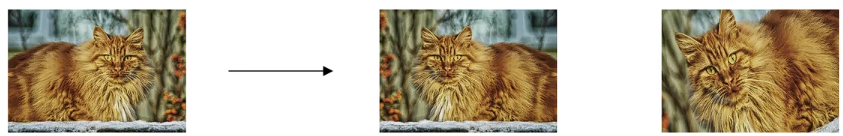
\includegraphics[width=12cm]{14.png}
            
\includegraphics[width=12cm]{15.png}
        \end{figure}
        \item Early stopping can be used to prevent overfitting from happening
        \begin{itemize}
            \item If the NN is overfitting the data, the dev set error will initially decrease before increasing
            \item Training of the NN can be stopped when the dev set error is lowest and the data has not been overfit
        \end{itemize}
        \item Using early stopping links the task of optimizing $J$ and not overfitting the data
        \begin{itemize}
            \item Early stopping will prevent the cost function from being optimized 
        \end{itemize}
        \item L2 regularization is a better method to prevent overfitting
        \begin{itemize}
            \item Requires a choice for the value of $\lambda$ and is much more computationally expensive
        \end{itemize}
    \end{itemize}
    \subsubsection{Setting up the Optimization Problem}
    \begin{itemize}
        \item Normalization can be used to speed up the training of a NN
        \begin{itemize}
            \item Subtract the mean:
            $$\mu=\frac{1}{m}\sum_{i=1}^mx^{(i)}$$
            $$x:=x=\mu$$
            \item Normalize the variance:
            $$\sigma^2=\frac{1}{m}\sum_{i=1}^mx^{(i)}**2$$ 
            $$x/=\sigma$$
        \end{itemize}
        \item When normalizing a training set, test set and training set should be processed together
        \begin{itemize}
            \item All the data must go through the same transformation
        \end{itemize}
        \item For data that is not normalized, the cost function will be very elongated
        \begin{itemize}
            \item The gradient will be quite shallow and will take longer to converge
            \item Algorithm will require a smaller learning rate
            \vspace{5mm}
            \begin{figure}[ht]
                \centering
                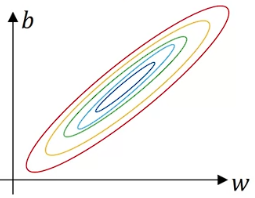
\includegraphics[width=8cm]{18.png}
            \end{figure}
        \end{itemize}
        \item On average, normalized data will have a cost function that is more symmetric
        \begin{itemize}
            \item Gradient descent will converge faster and can use a larger learning rate
            \begin{figure}[ht]
                \centering
                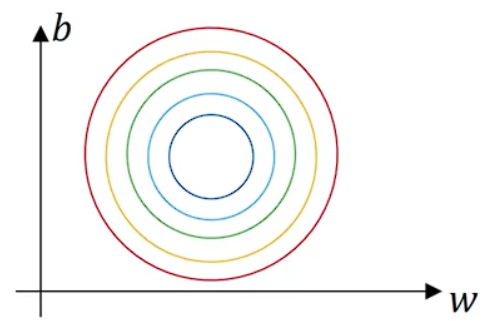
\includegraphics[width=8cm]{19.png}
            \end{figure}
        \end{itemize}
    \end{itemize}

    \vspace{5mm}
    \textbf{Vanishing/Exploding Gradients}
    \begin{itemize}
        \item For very deep neural networks, the derivatives can get exponentially big or small
        \item If the weights of a NN are all the same, the prediction $\hat{y}$ will $x$ to the $L$th power
        \begin{itemize}
            \item For $W^{[l]}>I$ the gradient will explode
            \item For $W^{[l]}<I$ the gradient will vanish
        \end{itemize}
        \item Some modern applications use 152 layer NN
        \begin{itemize}
            \item Require careful initialization of the weights to ensure correct training
        \end{itemize}
        \item For a single neuron:
        \begin{itemize}
            \item The output $\hat{y}$ will be the sum of all $w_ix_i$
            $$z = w_1x_1+w_2x_2+...+w_nx_n$$
            \item For a large $n$, want a smaller $w_i$
            \item Want $\text{Var}(w_i)=\frac{1}{n}$
        \end{itemize}
        \begin{minted}[escapeinside=||]{Python}
    |$W^{[l]}$| = np.random.randn(shape) * np.sqrt|$\left(\frac{1}{n^{[l-1]}}\right)$|
        \end{minted}
        \begin{itemize}
            \item Variance of Gaussian random variable can be set by multiplying by sqrt tem
        \end{itemize}
        \item For ReLU activation function, the variance should be set to $\frac{2}{n}$
        \begin{itemize}
            \item tanh activation uses Xavier initialization $\frac{1}{n^{[l-1]}}$
            \item Yoshua Bengio multiplied random variable by $\sqrt{\frac{2}{n^{[l-1]}+n^{[l]}}}$
        \end{itemize}
        \item Initialization of weights aims to set weight matrices close to 1
        \begin{itemize}
            \item Helps to prevent $\hat{y}$ from vanishing or exploding too quickly
        \end{itemize}
        \item Variance parameter can be tuned as another hyperparameter
    \end{itemize}
    \end{document}